                %%%%%%%%%%%%%%%%%%%%%%%%%%%%%%%%%%%%%%%%%%%%%%%%%%%%%%%%%%%%%%%%%%%%%%%%%%%%%%%%%%%%%%%%%%%%%%
% Template Beamer Sugestivo para Projetos no Senac
% by ezefranca.com
% Based on MIT Beamer Template
% As cores laranja e azul seguem o padrao proposto no manual de uso da identidade visual senac
%%%%%%%%%%%%%%%%%%%%%%%%%%%%%%%%%%%%%%%%%%%%%%%%%%%%%%%%%%%%%%%%%%%%%%%%%%%%%%%%%%%%%%%%%%%%%% 

%\documentclass{beamer} %voce pode usar este modelo tambem
\documentclass[handout,t]{beamer}
\usepackage{graphicx,url}
\usepackage[english]{babel}   
\usepackage[utf8]{inputenc}
\usepackage[square,numbers,sort&compress]{natbib}
\batchmode
% \usepackage{pgfpages}
% \pgfpagesuselayout{4 on 1}[letterpaper,landscape,border shrink=5mm]
\usepackage{amsmath,amssymb,enumerate,epsfig,bbm,calc,color,ifthen,capt-of}
\usetheme{Berlin}
\usecolortheme{senac}
\usepackage{graphicx}
\graphicspath{ {images/} }

\usepackage{biblatex}
\usepackage{filecontents}
\begin{filecontents*}{general.bib}
@misc{A01,
  author = {Author, A.},
  year = {2001},
  title = {Alpha},
}
@misc{B02,
  author = {Buthor, B.},
  year = {2002},
  title = {Bravo},
}
\end{filecontents*}

\addbibresource{general.bib}

\nocite{*}


%-------------------------Titulo/Autores/Orientador------------------------------------------------
\title[Final Project]{Planning graph characterization through structural properties}
\date{December 12 2017}
\author{Jos\'e Anastacio Hern\'andez Saldaña}
\institute[PISIS-FIME-UANL] % Your institution as it will appear on the bottom of every slide, may be shorthand to save space
{
Facultad de Ingenier\'ia Mec\'anica y El\'ectrica\\ % Your institution for the title page
\medskip
\textit{jose.hernandezsld@uanl.edu.mx} % Your email address
}

%-------------------------Logo na parte de baixo do slide------------------------------------------
\pgfdeclareimage[height=0.7cm]{senac-logo}{senac-logo.pdf}
\logo{\pgfuseimage{senac-logo}\hspace*{0.5cm}}

%-------------------------Este código faz o menuzinho bacana na parte superior do slide------------
\AtBeginSection[]
{
  \begin{frame}<beamer>
    \frametitle{Outline}
    \tableofcontents[currentsection]
  \end{frame}
}
\beamerdefaultoverlayspecification{<+->}
% -----------------------------------------------------------------------------
\begin{document}
% -----------------------------------------------------------------------------

%---Gerador de Sumário---------------------------------------------------------
\frame{\titlepage}
\section[]{}
\begin{frame}{Summary}
  \tableofcontents
\end{frame}
%---Fim do Sumário------------------------------------------------------------


% -----------------------------------------------------------------------------
\section{Introduction}
\begin{frame}{Introduction}
%introducao
This is a reseach based in the analysis of the planning graphs from
the GraphPlan algorithm, an algoritm that creates a planning graph structure in a polynomial time. Planning problems are in the complexity class \textit{PSPACE-complete}, to solve a planning problem is needed at least a polynomial amount of space. The study of the planning problems can help to improve the planner performance with reasonable resources.
\\
This work tries to identify structural properties through the graph analysis of the planning graphs from the problems stablish in the International Planning Competition (IPC) from 1998 and using the result to corroborate the analysis.


\end{frame}
%------------------------------------------------------------------------------

%------------------------------------------------------------------------------
\section{Automated Planning}
\begin{frame}{Automated Planning}
  
  \textit{Automated planning} studies studies how to emulate the human
  reasoning side of acting. A planning problem is based on a model of
  the environment, where the initial conditions are the description of
  that environment including the objects in it and their descriptions,
  a set of available actions, where each action requires a set of
  conditions to be fulfilled before can be carried out, and a goal,
  that captures the conditions to be fufilled by the secquence of
  actions, this sequence is know as the plan and the planning solver
  is known as the planner.
  

\end{frame}
%------------------------------------------------------------------------------
%------------------------------------------------------------------------------
\subsection{Classical Planning}
\begin{frame}{Classical Planning}
  
  There exists a lot of automated planning problem forms based on assumption
restrictions about the way of modeling a environment, the
restricted model of automated planning consists in the
following restriction assumptions.

\end{frame}

\begin{frame}
\begin{itemize}
\item[\textbf{A0}] Finite: The system has a finite set of states.
\item[\textbf{A1}] Fully observable: one completely knows the state of the system.
\item[\textbf{A2}] Deterministic: every action takesjust to a one state.
\item[\textbf{A3}] Static: the system stays in the
  same state until an action is taken, there are no outside actions or
  further events.
\item[\textbf{A4}] Restricted goals: the planner just tries to reach
  the final state, avoiding certain states or utility functions are
  not handled.
\item[\textbf{A5}] Sequential Plans: The solution plan is an ordered
  finite sequence of actions
\item[\textbf{A6}] Implicit Time: Actions have no duration, the state
  transition is immediate.
\item[\textbf{A7}] Offline planning: The planner is concerted about
  system while the planning process is being performed, there
  is no system supervision or new and restricted actions or variables
  after the initial state.
\end{itemize}
  

\end{frame}
\subsection{GraphPlan}
\begin{frame}{GraphPlan}
  
The two of the most used planners to solve automated classical planning
problems are GraphPlan  and SATPLAN and both are equally expresive,

Planning as satisfability (SATPLAN), consist in represent the planning
conditions as a Propositional Satisfiability Problem, while GraphPlan
uses a a directed, leveled graph with two kinds of nodes and three
kinds of edges.

These two structures of represent the planning classical problems were
the principal influence in the IPC of 1998, and all the planners were
based in one of them.

\end{frame}

\subsection{The International Planning Competition}
\begin{frame}{IPC}  

The International Planning Competition (IPC) is organized by the
International Conference on Automated Planning and Scheduling (ICAPS)
since 1998 and reunites planners developed by researchers from all
over the world to create planning domains problems and to make a
comparison among existing planners and measure the progress in the
field.

\end{frame}
%------------------------------------------------------------------------------
\section{Computational Complexity}
\begin{frame}{Computational Complexity}
In computer science, the study of the use of resource needed to
execute an algorithm is known as algorithm analysis and the study of
how to describe a problem in terms of computational resources used to
solve it is known as computational complexity. The
computational complexity uses a series of classes known as complexity
classes where a set of problems is categorized based on the resources
required to solve it.
\end{frame}
%------------------------------------------------------------------------------
\section{Metodology}
\begin{frame}{Metodology}
  The methodology of the present work consists in studying the
  benchmark problems proposed in the IPC using the planning graphs
  generated from the GraphPlan algorithm, to identify graph properties
  that are factors in the algorithms solver performance reported in
  the IPC and identify structural properties among problems to
  categorize them and establish metrics asds.
\end{frame}
%------------------------------------------------------------------------------

%------------------------------------------------------------------------------

\begin{frame}
  \begin{table}[h!]
    \centering
    \begin{tabular}{c c c c}  
      Domain & Problems & Solved & Graph \\ [0.5ex] 
      \hline \hline
      assembly  & 30 & 0 & 0   \\
      gripper   & 30 & 3 & 30  \\
      logistics & 30 & 10 & 30 \\
      movie     & 30 & 30 & 30 \\
      mprime    & 30 & 23 & 30 \\
      mystery   & 30 & 19 & 30 \\
      \hline
    \end{tabular}
    \caption{Domains used by competiton}
    \label{table:domaincompetition}
  \end{table}
\end{frame}
%------------------------------------------------------------------------------
\section{Results}
\begin{frame}{Results}
  \begin{figure}[ht!]
    \centering
    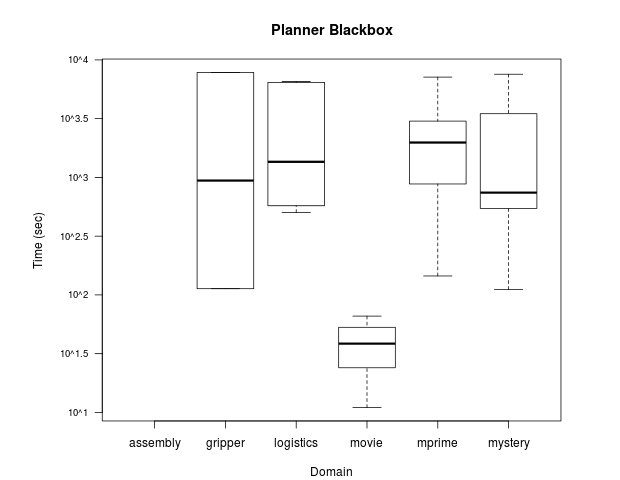
\includegraphics[width=0.75\linewidth]{bxplt_BB_Domain_Time}
%    \caption{BlackBlox Results}
    \label{fig::figura1} 
  \end{figure}  
\end{frame}
\begin{frame}
  \begin{figure}[ht!]
    \centering
    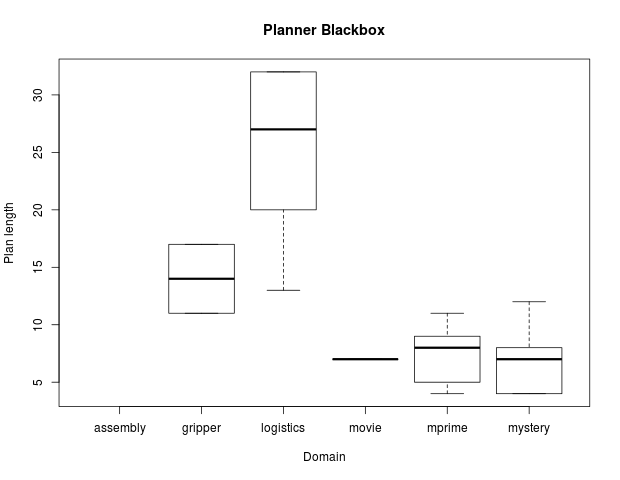
\includegraphics[width=0.75\linewidth]{bxplt_BB_Domain_length}
%    \caption{BlackBlox Results}
    \label{fig::figura2} 
  \end{figure}    
\end{frame}
\begin{frame}
  \begin{figure}[ht!]
    \centering
    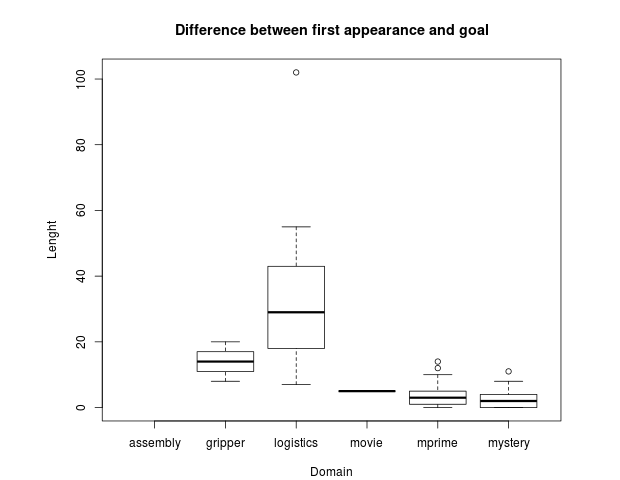
\includegraphics[width=0.75\linewidth]{bxplt_FirstApp_Domain}
%    \caption{BlackBlox Results}
    \label{fig::figura9} 
  \end{figure}    
\end{frame}

\begin{frame}
  \begin{figure}[ht!]
    \centering
    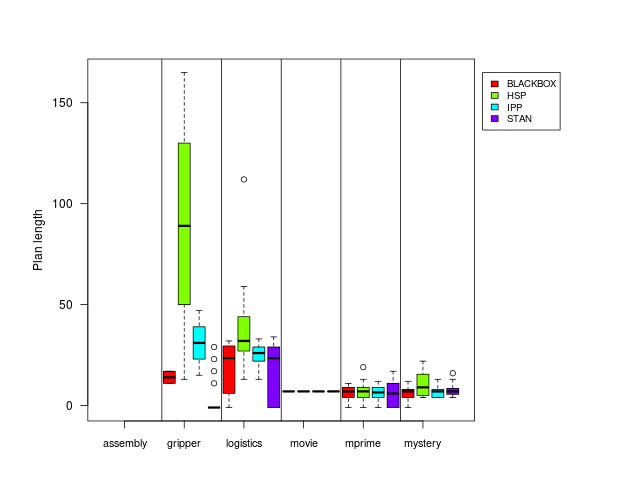
\includegraphics[width=0.75\linewidth]{bxplt_All_GDomain_Planner_lenght}
%    \caption{BlackBlox Results}
    \label{fig::figura3} 
  \end{figure}  
\end{frame}
\begin{frame}
  \begin{figure}[ht!]
    \centering
    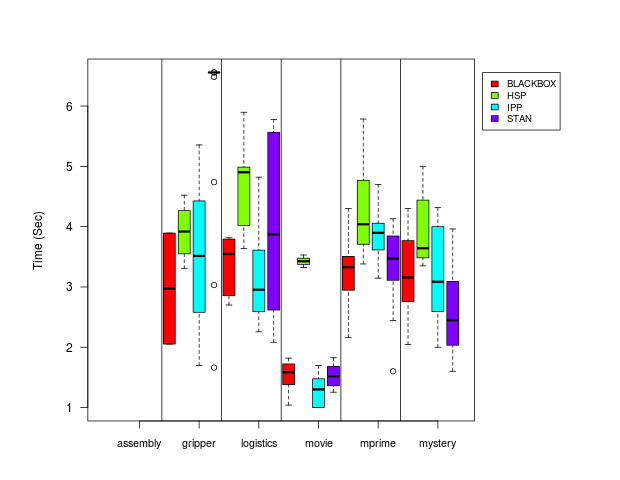
\includegraphics[width=0.75\linewidth]{bxplt_All_GDomain_Planner_Time}
%    \caption{BlackBlox Results}
    \label{fig::figura4} 
  \end{figure}    
\end{frame}

\begin{frame}
  \begin{figure}[ht!]
    \centering
    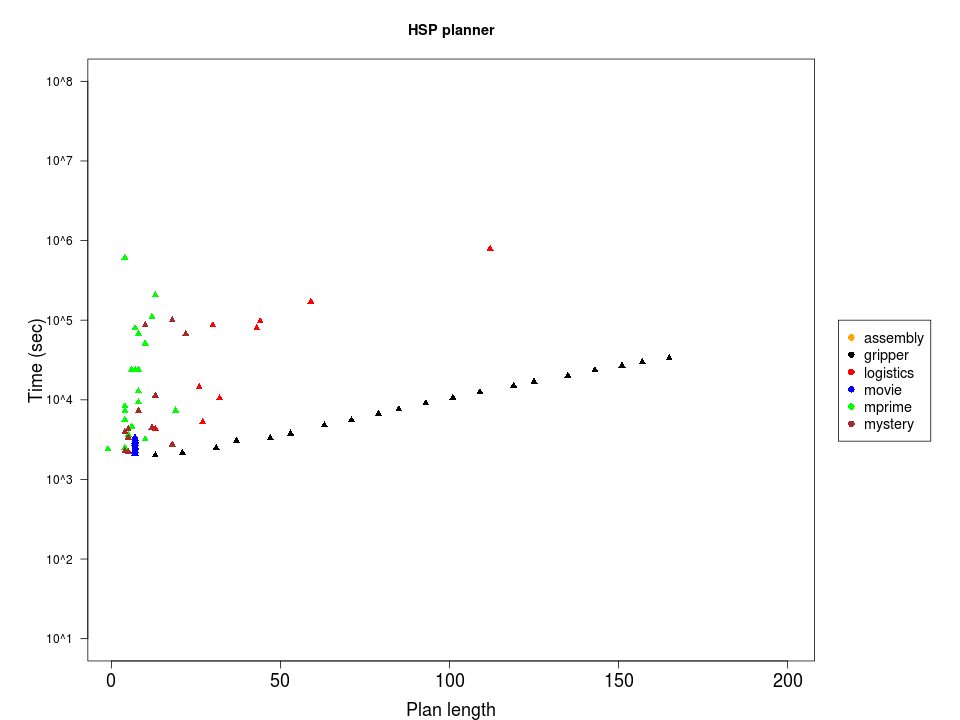
\includegraphics[width=0.75\linewidth]{bxplt_HSP_Time_length}
    \label{fig::figura5} 
  \end{figure}      
\end{frame}

\begin{frame}
  \begin{figure}[ht!]
    \centering
    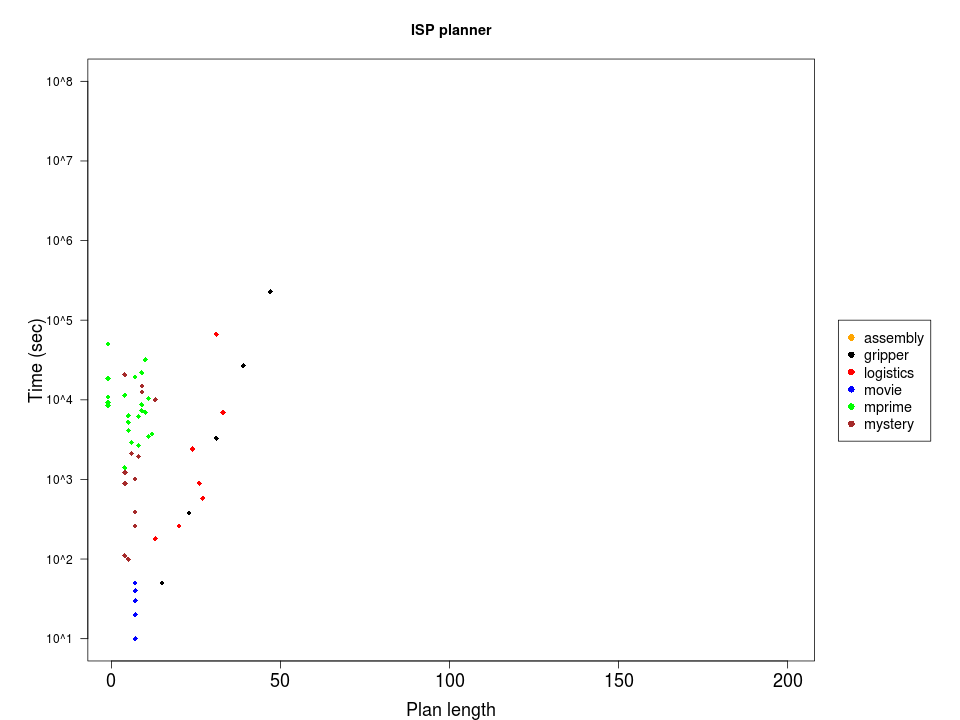
\includegraphics[width=0.75\linewidth]{bxplt_ISP_Time_length}
    \label{fig::figura6} 
  \end{figure}        
\end{frame}

\begin{frame}
  \begin{figure}[ht!]
    \centering
    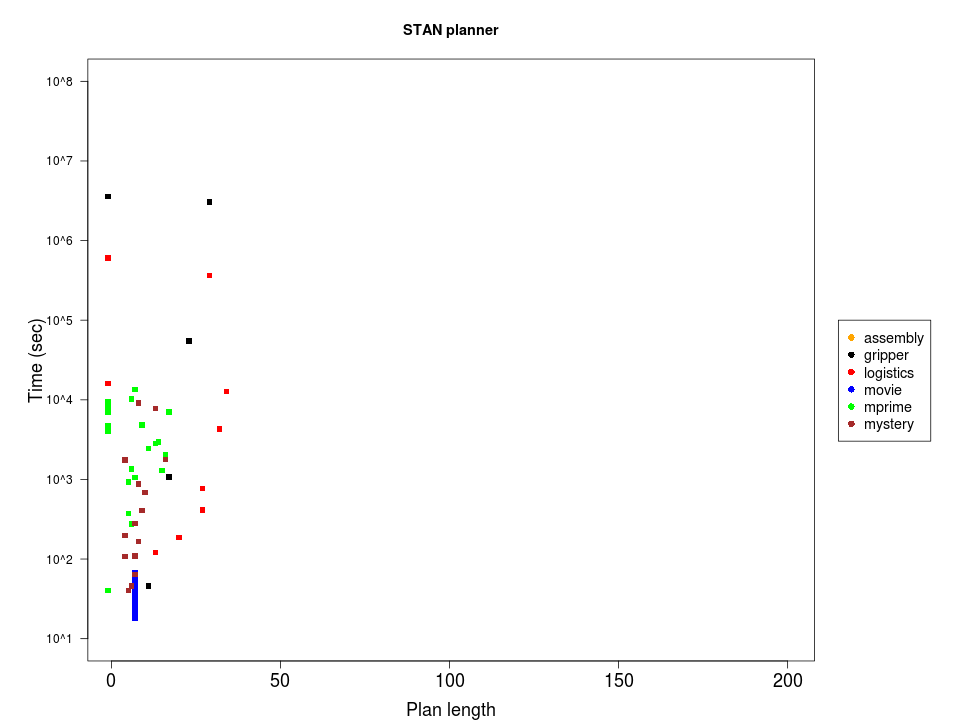
\includegraphics[width=0.75\linewidth]{bxplt_STAN_Time_length}
    \label{fig::figura7} 
  \end{figure}        
\end{frame}

\begin{frame}
  \begin{figure}[ht!]
    \centering
    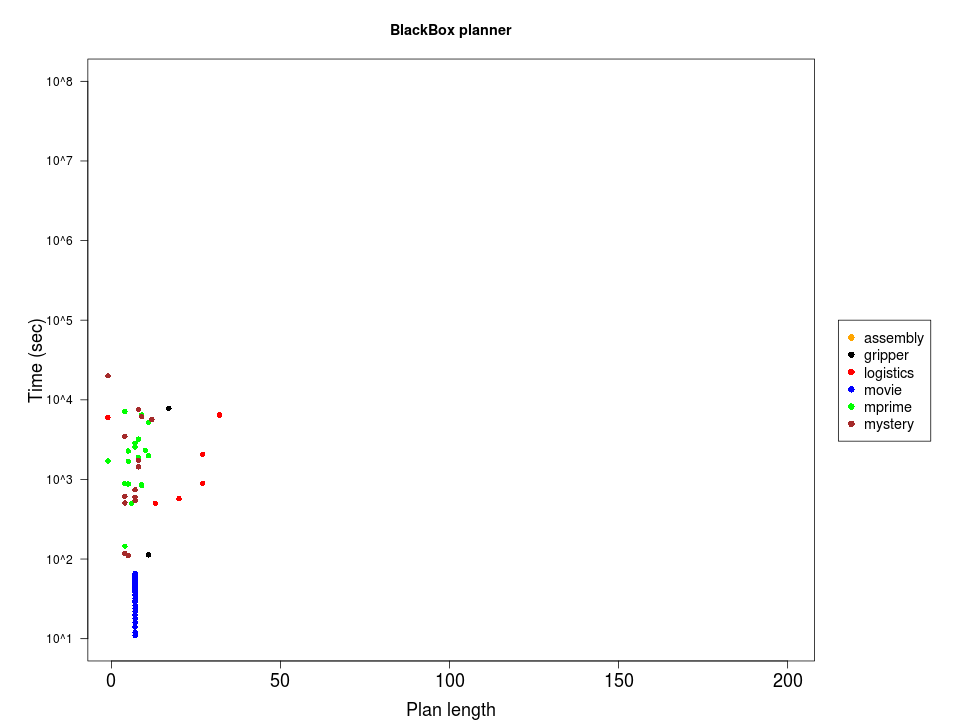
\includegraphics[width=0.75\linewidth]{bxplt_BB_Time_length}
    \label{fig::figura8} 
  \end{figure}        
\end{frame}

\begin{frame}
  \begin{figure}[ht!]
    \centering
    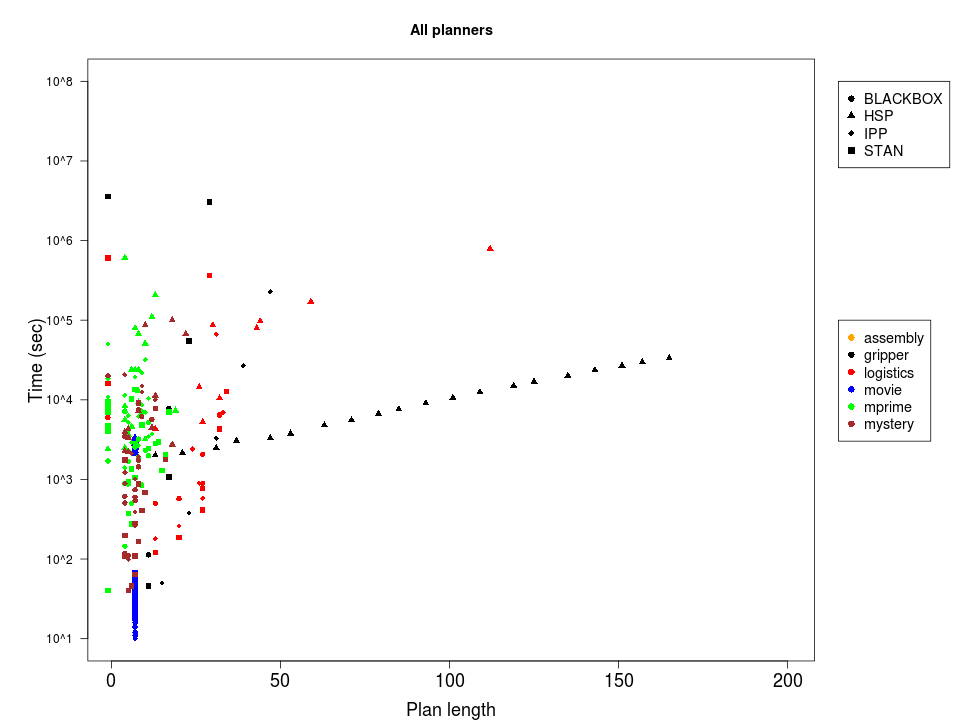
\includegraphics[width=0.75\linewidth]{bxplt_All_Time_length}
    \label{fig::figura10} 
  \end{figure}        
\end{frame}


\begin{frame}
  \begin{figure}[ht!]
    \centering
    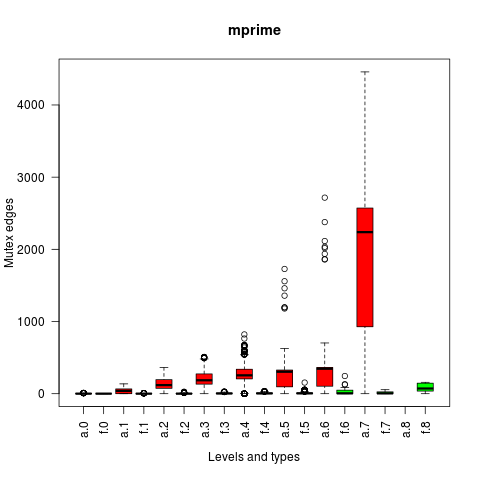
\includegraphics[width=0.65\linewidth]{dist_exlusive_mprime}
    \label{fig::figura12} 
  \end{figure}        
\end{frame}


\begin{frame}
  \begin{figure}[ht!]
    \centering
    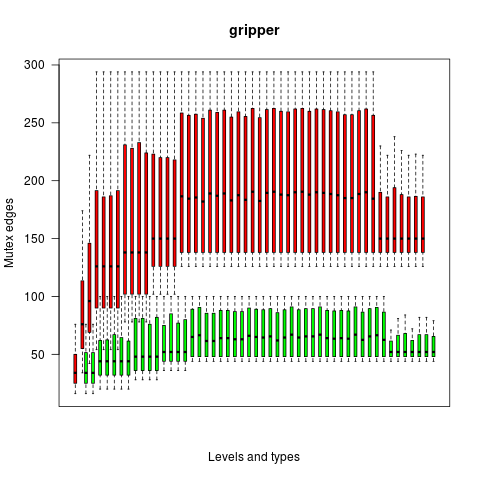
\includegraphics[width=0.65\linewidth]{dist_exlusive_gripper}
    \label{fig::figura12} 
  \end{figure}        
\end{frame}
%------------
%------------------------------------------------------------------------------
%\section{References}
%\begin{frame}{References}
%  \printbibliography
%  \bibliographystyle{plain}
%  \bibliography{general.bib}
%\end{frame}
%------------------------------------------------------------------------------

%------------------------------------------------------------------------------
%\section{Agradecimentos}
%\begin{frame}{Agradecimentos}
%Agradeço a todos que colaboraram  para realizaç~ao deste projeto.
%Agradeço ao Alexandre Bencz pelo assembly de cada dia.
%Agradeço ao Sonata Arctica, Avantasia, Mago de Oz, Cain's Offering, e todas as outras bandas de Power Metal.    
%\end{frame}
%------------------------------------------------------------------------------

%------------------------------------------------------------------------------
%\subsection{Sites legais}
%\begin{frame}{Sites legais}
%  Want to know more? See!
%  \begin{itemize}
%    \item Browse in my page \url{http://www.ezefranca.com}.
%    \item Browse on BCC page \url{http://www.sp.senac.br/bcc}.
%    \item Thanks WriteLaTeX from Support! \url{http://www.writelatex.com}.
%  \end{itemize}
%  
%\end{frame}
%------------------------------------------------------------------------------

% -----------------------------------------------------------------------------
\end{document}
%-----------------------------------------------Este comentario nunca aparecera
